\chapter{Desarrollo, resolución, resultados e interpretación}

\section{¿Aumenta la pareja el número de faltas en clase?}
En nuestro dataset una proporción considerable de alumnos están en una relación amorosa.

\begin{figure}[H]
    \centering
    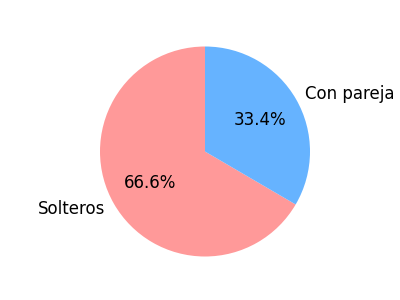
\includegraphics[width=0.6\textwidth]{./figures/proporcion-solteros-pareja.png}
    \caption{Proporción de alumnos solteros vs con pareja}
    \label{fig:prop-solteros}
\end{figure}

\pagebreak

Además, vemos que la edad de los estudiantes está comprendida entre los 15 y 22 años. Podemos suponer que en estas edades las relaciones románticas tenga mucho impacto en la vida escolar, en concreto en la asistencia en clase.
\begin{figure}[H]
    \centering
    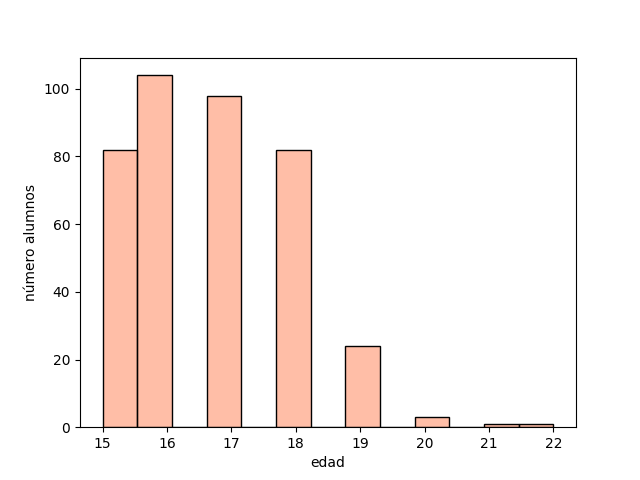
\includegraphics[width=0.8\textwidth]{./figures/edad-alumnos.png}
    \caption{Histograma de las edades de los alumnos}
    \label{fig:hist-edad}
\end{figure}

Por lo tanto, con el objetivo de estudiar que factores de la vida personal de los alumnos influyen en sus notas escolares, vamos a comenzar contrastando si el hecho de tener pareja aumenta el número de faltas en clase.
\begin{equation*}
    \begin{split}
        & X \equiv \text{Número de faltas en clase de los alumnos con pareja}\\
        & Y \equiv \text{Número de faltas en clase de los alumnos solteros}
    \end{split} 
\end{equation*}

\pagebreak

Para poder elegir un contraste de hipótesis, primero debemos estudiar la distribución de los datos.

Viendo los gráficos de distribución de el número de faltas en clase de los alumnos con pareja y solteros podemos asumir que los datos no provienen de una población normal, ya que en ambos casos son datos muy asimétricos.

\begin{figure}[H]
    \centering
    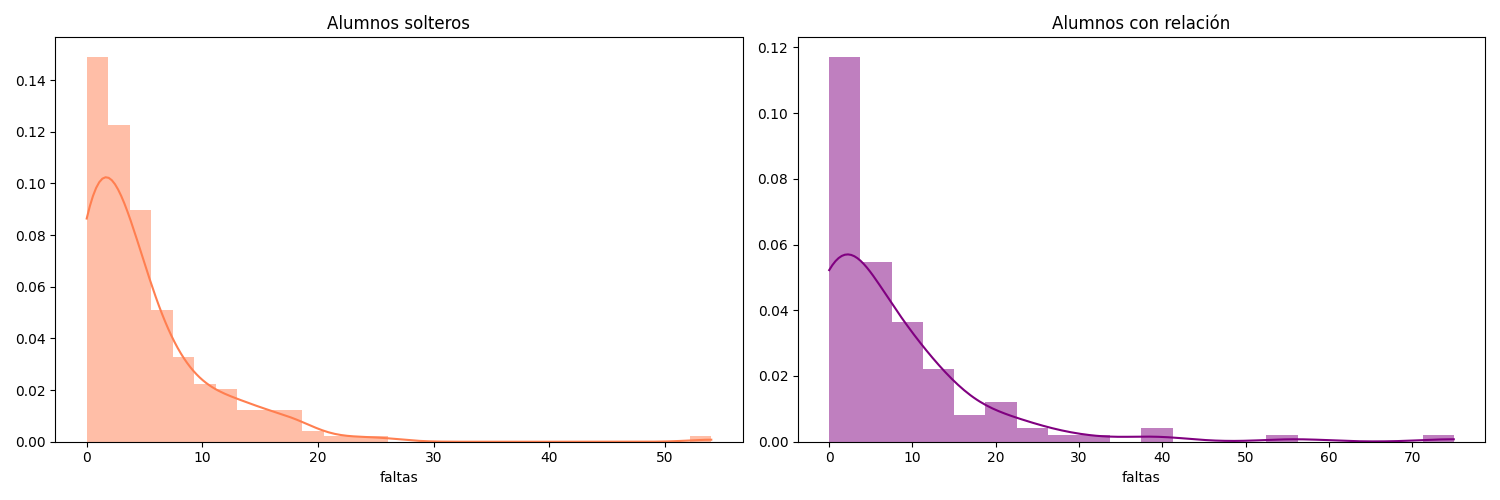
\includegraphics[width=1\textwidth]{./figures/distribucion-numero-faltas.png}
    \caption{Gráficos de distribución del número de faltas de los alumnos}
    \label{fig:dist-num-faltas}
\end{figure}

Para asegurarnos de que estamos en lo correcto realizaremos un contraste de normalidad. En nuestro caso utilizaremos el test Ómnibus d´Agostino, ya que nuestros datos cumplen con el requisito de tener más de 20 entradas ($n>20$).

Realizaremos el test tanto para alumnos solteros como para alumnos con pareja. Las hipótesis para los alumnos solteros serían las siguientes:

\begin{itemize}
    \item \textbf{Hipótesis nula ($H_0$)}: $X \sim N(\mu, \sigma)$ (Los datos del número de faltas en alumnos con pareja siguen una distribución normal)
    \item \textbf{Hipótesis alternativa ($H_a$)}: $X \not \sim N(\mu, \sigma)$ (Los datos del número faltas en alumnos con pareja no sigue una distribución normal)
\end{itemize}

\pagebreak

En el caso de los alumnos con pareja al calcular el estadístico de contraste observado obtenemos $K^2_x = 116.45$ y al calcular el p-valor obtenemos un valor muy cercano al cero.

\begin{equation*}
    \text{p-valor} = P(K^2_x > 116.45) \approx 0
\end{equation*}

Por lo tanto, en el caso de los alumnos solteros, los datos muestran evidencias suficientes para rechazar la hipótesis nula de que el número de faltas en la muestra sigue una distribución normal.

En el caso de los alumnos con pareja obtendremos las mismas conclusiones, por lo que aceptaremos la no-normalidad de los datos en ambos casos.
\pagebreak

Como asumimos que los datos no provienen de una distribución normal utilizaremos un contraste no paramétrico. Como estamos trabajando con muestras independientes, eligiremos el contraste U de Mann-Whitney.

Para ello plantearemos las siguientes hipótesis:

\begin{itemize}
    \item \textbf{Hipótesis nula ($H_0$)}: $\mu_x = \mu_y$ (No existe una diferencia significativa entre el número de faltas medio entre los alumnos con pareja y solteros)
    \item \textbf{Hipótesis alternativa ($H_a$)}: $\mu_x > \mu_y$ (El número de faltas medio en los alumnos con pareja es mayor que el de los alumnos solteros)
\end{itemize}

Al cálcular es estadístico de contraste $U$ obtenemos un valor observado de 18787.5, el cual sugiere diferencias pequeñas entre ambas poblaciones.
\begin{equation*}
    \text{p-valor} = P(U > 18787.5) = 0.0874 > \alpha 
\end{equation*}

Viendo que el p-valor supera nuestro nivel de significación $\alpha$ de 0.05, podemos afirmar que al $5\%$ los datos no muestran evidencias suficientes como para rechazar la hipótesis de que no exista una diferencia significativa entre el número de faltas medios de los alumnos solteros y con pareja. 

Este resultado es sorprendente ya que la media faltas en solteros es de $4.84$ faltas y en alumnos con pareja es de $7.44$ faltas. 
\begin{equation*}
    \begin{split}
        & \bar{x} = 7.44\\
        & \bar{y} = 4.84
    \end{split}
\end{equation*}

Pero en definitiva, aceptamos que el hecho de tener pareja no afecta significativamente al número de faltas medio a lo largo del curso.

\pagebreak

\section{¿Mejoran las notas a lo largo del curso?}

Un indicio de un buen sistema educativo es el de que los alumnos mejoran sus notas a lo largo del curso. En nuestros datos tenemos registros de las notas de los estudiantes a lo largo del curso, por lo tanto podemos contrastar si existe un progreso. Para ello contrastaremos si la nota media del primer periodo $G_{1}$ y la nota media final $G_{3}$ difieren significativamente.

\begin{equation}
    \begin{split}
        & X \equiv \text{Nota de los alumnos en el primer periodo}\\
        & Y \equiv \text{Nota final de los alumnos}
    \end{split} 
\end{equation}

Esta vez vemos que los gráficos de distribución de las notas del primer periodo y del final se asemejan más al de la distribución normal.

\begin{figure}[H]
    \centering
    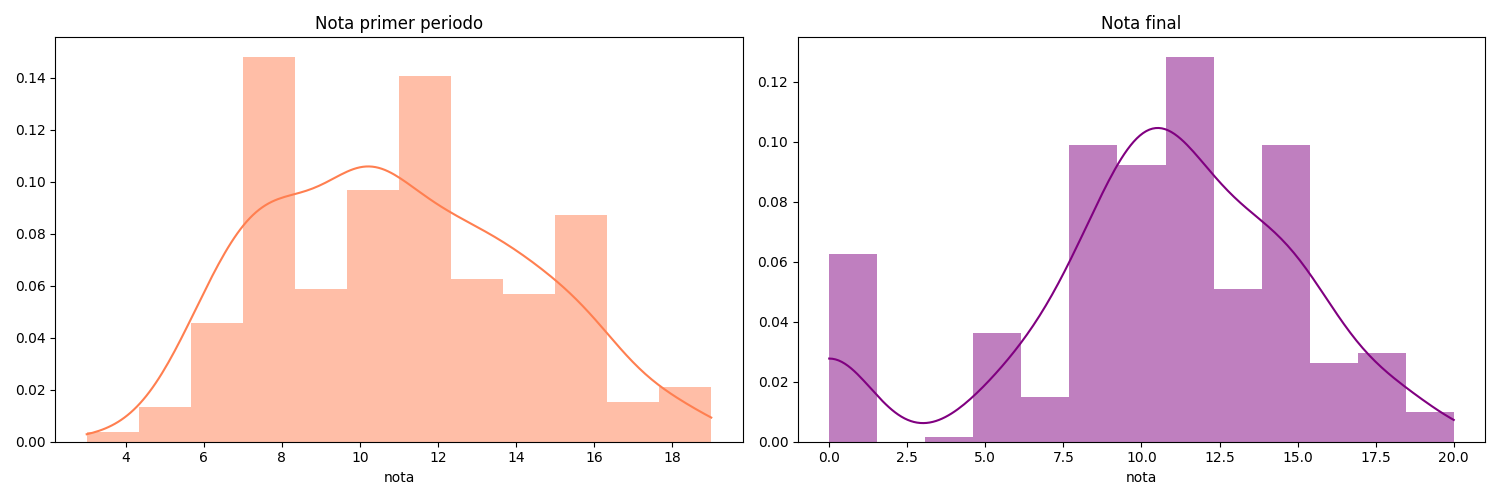
\includegraphics[width=1\textwidth]{./figures/dist-notas-alumnos.png}
    \caption{Gráficos de distribución de las notas de los alumnos}
    \label{fig:dist-notas}
\end{figure}

Si volvemos a realizar el test de Ómnibus d´Agostino obtenemos los siguientes resultados:
\begin{equation*}
    \begin{split}
        & K^2_{x} = 22.61 \Rightarrow \text{p-valor} = P(K^2 > 22.61) \approx 0\\ 
        & K^2_{y} = 32.05 \Rightarrow \text{p-valor} = P(K^2 > 32.05) \approx 0
    \end{split}
\end{equation*}

Aunque los estádisticos observados son más pequeños (denotando que las muestras son más anteriores que cuando veíamos las faltas en clase), los p-valor siguen siendo muy cercanos al cero.

\pagebreak

Sin embargo, como los datos son medianamente simétricos y además disponemos de una muestra suficientemente grande, utilizaremos un contraste paramétrico de diferencia de medias.
\begin{equation*}
    \begin{split}
        & \gamma_{1}(x) = \frac{\sum_{i=1}^{n}(x_i - \bar{x})^3}{n \cdot s^3} = 0.24\\
        & \gamma_{1}(y) = \frac{\sum_{i=1}^{n}(y_i - \bar{y})^3}{n \cdot s^3} = -0.73
    \end{split} 
\end{equation*}

Como estamos trabajando con muestras dependientes (medimos la nota del alumno en distintos momentos y además la nota final depende de la nota del primer y segundo periodo), utilizaremos un t-test de muestras pareadas.
\begin{itemize}
    \item \textbf{Hipótesis nula ($H_0$)}: $\mu_x - \mu_y = \mu_D = 0$ (no existe diferencias significativas entre la nota media del primer periodo y la nota media final)
    \item \textbf{Hipótesis alternativa ($H_a$)}: $\mu_x - \mu_y = \mu_D > 0$ (la nota media final mejora significativamente respecto a la nota media del primer periodo)
\end{itemize}

Al realizar el test obtenemos los siguientes resultados:
\begin{equation*}
    t_{obs} = 3.55 \Rightarrow \text{p-valor} = P(t_{394} > 3.55) = 0.0002
\end{equation*}

Por lo tanto, viendo que el p-valor es pequeño, concluimos que los datos muestran evidencias suficientes como para rechazar que la diferencia entre la media del primer periodo y la media final no es significativa. Aceptaremos la hipótesis alternativa de que la media final aumenta respecto a la del primer periodo.
